% from https://chat.stackexchange.com/transcript/message/43426419#43426419
\documentclass{standalone}

\usepackage{xcolor}
\usepackage{graphicx}
\usepackage{tikzducks}
\usepackage{marvosym}

\definecolor{linen}{HTML}{F3EAD8}
\definecolor{gold}{HTML}{CFB53B}
\definecolor{ruby}{HTML}{E0115F}

\newcommand{\AnkhC}[1][1]{%
\scalebox{#1}{%
\begin{tikzpicture}
  \begin{scope}[scale=0.08]
    \path [fill=ruby] (0,0) [bend left=75] to (0,1) [bend left=75] to cycle;
  \end{scope}
  \begin{scope}[yshift=-1.1,scale=#1]
    \node {\color{gold}\Ankh};
  \end{scope}
\end{tikzpicture}}}

\makeatletter
\def\mummy@distance{0.12}
\def\mummy@color{black}
\def\mummy@rotate{-90}
\def\mummy@initialx{0.1}
\def\mummy@initialy{-0.3}
\def\mummy@width{0.01}
\def\mummy@height{2.7}
\def\mummy@emblem{\AnkhC[2.5]}
\def\mummy@stripes{%
\foreach \shifta in {0,\mummy@distance,...,2.4}{%
  \fill[\mummy@color,rotate around={\mummy@rotate:(1.2,0.9)}]
  ($(\mummy@initialx,\mummy@initialy)+(\shifta,0)$) rectangle ($(\mummy@initialx,\mummy@initialy)+(\shifta,0)+(\mummy@width,\mummy@height)$);
}%
}

\begin{document}
\pagenumbering{gobble}
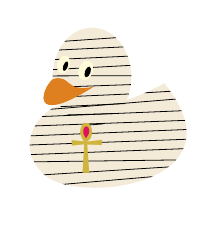
\begin{tikzpicture}
\duck[body=linen]
\path (0.1,0.1) rectangle (2.1,1.45);
\begin{pgfinterruptboundingbox}
  \begin{scope}
    \clip (0.90,1.50) ellipse (0.50 and 0.625);
\foreach \shifta in {0,\mummy@distance,...,2.4}{%
  \fill[\mummy@color,rotate around={{-90+5*rnd}:(1.2,0.9)}]
  ($(\mummy@initialx,\mummy@initialy)+(\shifta,0)$) rectangle ($(\mummy@initialx,\mummy@initialy)+(\shifta,0)+(\mummy@width,\mummy@height)$);
}%
  \end{scope}
  \begin{scope}
    \clip \duckpathbody;
\foreach \shifta in {0,\mummy@distance,...,2.4}{%
  \fill[\mummy@color,rotate around={{-90+5*rnd}:(1.2,0.9)}]
  ($(\mummy@initialx,\mummy@initialy)+(\shifta,0)$) rectangle ($(\mummy@initialx,\mummy@initialy)+(\shifta,0)+(\mummy@width,\mummy@height)$);
}%
  \end{scope}
  \fill[\duck@bill] \duckpathbill;
    % right eye %%%%%%%%%%%%%%%%%%%%%%%%%%%%%%%%%%%%%%%%%%%%%%%%%%%%%%%%%%
  \fill[\duck@eye, rotate=-20] 
    (0.23,1.7675) ellipse (0.0893 and 0.125);
  \fill[\duck@pupil, rotate=-20] 
    (0.26,1.7575) ellipse (0.0357 and 0.0714);
  % left eye %%%%%%%%%%%%%%%%%%%%%%%%%%%%%%%%%%%%%%%%%%%%%%%%%%%%%%%%%%%
  \fill[\duck@eye, rotate=-20] 
    (-0.06,1.74) ellipse (0.0786 and 0.1143);
  \fill[\duck@pupil, rotate=-20] 
    (-0.03,1.73) ellipse (0.0286 and 0.0643);
\end{pgfinterruptboundingbox}
\node[xshift=1,yshift=-3] at (wing) {\mummy@emblem};

%% from https://tex.stackexchange.com/a/409386/121799
%\path[rotate=-20]
%    (0.23,1.7675)coordinate(ECR) ellipse (0.0893 and 0.125);
%
%\path[rotate=-20]
%    (-0.06,1.74)coordinate(ECL) ellipse (0.0786 and 0.1143);
%
%\foreach \x/\y in {0/1,1/2,2/3,3/3.3,4/3,5/2,6/1.4}
%{ \draw[brown!50!black,rotate=-20,line cap=round] (ECR)--++(\x*15+220:0.11cm+\y*0.012cm); };
%
%\foreach \x/\y in {0/1,1/2,2/3,3/3.3,4/3,5/2,6/1.4}
%{ \draw[brown!50!black,rotate=-20,line cap=round] (ECL)--++(\x*15+220:0.11cm+\y*0.009cm); };
%%
%%
%\fill[rotate=-20,yellow!50!brown]
%    (0.23,1.7675) ellipse (0.0893 and 0.125);
%%
%\fill[rotate=-20,yellow!50!brown]
%    (-0.06,1.74) ellipse (0.0786 and 0.1143);
\end{tikzpicture}

\end{document}